\documentclass[11pt]{beamer}
\usepackage{listings} % Include the listings-package
\usepackage[T1]{fontenc}
\usepackage[utf8]{inputenc}
\usepackage[english]{babel}
\usepackage{amsmath}
\usepackage{amssymb, amsfonts, latexsym, cancel}
\usepackage{float}
\usepackage{graphicx}
\usepackage{epstopdf}
\usepackage{subfigure}
\usepackage{hyperref}
%\usepackage{authblk}
\usepackage{blindtext}
\usepackage{booktabs} % Allows the use of \toprule, 
\usepackage{filecontents}
\usepackage{courier} %% Sets font for listing as Courier.
\usepackage{listings}
%\usepackage{listings, xcolor}
\lstset{
tabsize = 2, %% set tab space width
showstringspaces = false, %% prevent space marking in strings, string is defined as the text that is generally printed directly to the console
numbers = left, %% display line numbers on the left
commentstyle = \color{green}, %% set comment color
keywordstyle = \color{blue}, %% set keyword color
stringstyle = \color{red}, %% set string color
rulecolor = \color{black}, %% set frame color to avoid being affected by text color
basicstyle = \small \ttfamily , %% set listing font and size
breaklines = true, %% enable line breaking
numberstyle = \tiny,
}
\usepackage{caption}
\DeclareCaptionFont{white}{\color{white}}
\DeclareCaptionFormat{listing}{\colorbox{gray}{\parbox{\textwidth}{#1#2#3}}}
\captionsetup[lstlisting]{format=listing,labelfont=white,textfont=white}
\definecolor{urlColor}{rgb}{0.06, 0.3, 0.57}
\definecolor{linkColor}{rgb}{0.57, 0.0, 0.04}
\definecolor{fileColor}{rgb}{0.0, 0.26, 0.26}
\hypersetup{
    colorlinks=true,
    linkcolor=linkColor,
    filecolor=fileColor,      
    urlcolor=urlColor,
}
\urlstyle{same}
\setbeamercovered{transparent}
%\usetheme{Boadilla}
\usetheme{CambridgeUS}
%\usetheme{Berkeley}
%\usetheme{Warsaw}
%\usetheme{Madrid}

\title[Interfaz de usuario]{\bf\Huge Shneiderman y Plaisant (2009)}
\subtitle{}

\author[Grupo 12]
{
	César Paul Vasquez Alvarez \\
	Christian Gonzalo Layme Fernandez \\
	Emerson Danny  Mendoza Hilasaca \\
	Edith Maricarmen Coaquira Cuevas  
}
\institute[UNSA]

\date[2020-09-15]{\scriptsize{2020-09-15}}
%\logo{
\includegraphics[width=3.0cm]{img/logo_unsa.jpg}}
\titlegraphic{
\includegraphics[width=2.0cm]{img/logo_unsa.jpg}}

\begin{document}

\begin{frame}
\titlepage
\end{frame}

\begin{frame}
\frametitle{Contenido}
\tableofcontents
\end{frame}

\section{Ben Shneiderman}
%References frame
\begin{frame}
\frametitle{Ben Shneiderman (n. 21 de agosto de 1947)}
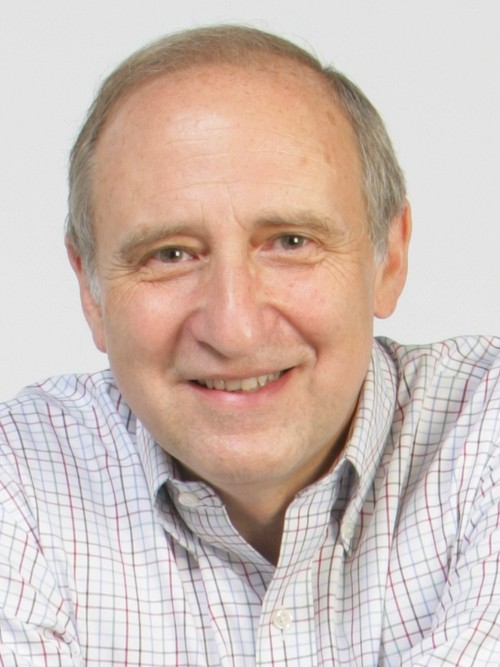
\includegraphics[width=3.0cm,height=3.0cm]{img/ben.jpg}\centering

\begin{itemize}
\item Catedrático de Informática en el Human-Computer Interaction Laboratory en la Universidad de Maryland en el College Park.
\item Su investigación principal está relacionada con la Interacción Persona-ordenador.
\end{itemize}
\end{frame}


\section{Catherine Plaisant}
%References frame
\begin{frame}
\frametitle{Catherine Plaisant (n. 26 de mayo de 1957)}
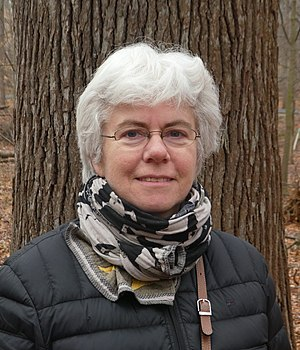
\includegraphics[width=3.0cm,height=3.0cm]{img/plaisant.jpg}\centering

\begin{itemize}
\item Científica de investigación en la Universidad de Maryland, College Park y subdirectora de investigación en Human-Computer Interaction Lab.
\item Contribuyó al desarrollo temprano de interfaces de pantalla táctil.
\item Sus trabajos se han centrado en herramientas de análisis visual para explorar patrones de secuencias de eventos temporales
\end{itemize}
\end{frame}

\section{Designing the User Interface: Strategies for Effective Human-Computer Interaction}
%References frame
\begin{frame}
\frametitle{Designing the User Interface: Strategies for Effective Human-Computer Interaction}
\begin{itemize}
\item Amplia cobertura de la participación en las redes sociales y el contenido generado por los usuarios. 
\item La participación en las redes sociales a través de varias técnicas de IHC sirve como mecanismos de apoyo poderosos pero de bajo costo. 
\item El concepto predominante de usabilidad universal subraya la necesidad crítica de atender las tecnologías de la información.
\item La facilidad del intercambio de información permite que amplias comunidades de usuarios produzcan grandes cantidades de contenido.
\end{itemize}
\end{frame}

\section{Ben Shneiderman y Catherine Plaisant}
%References frame
\begin{frame}
\frametitle{Ben Shneiderman y Catherine Plaisant}
\begin{itemize}
\item Lucha por la coherencia
\item Atiende a la usabilidad universal
\item ofrecer comentarios informativos
\item Diseñar flujos de tareas para lograr el cierre
\item Prevenir errores
\item Permitir una fácil reversión de acciones
\item Haga que los usuarios sientan que tienen el control
\item Minimizar la carga de memoria a corto plazo

\end{itemize}
\end{frame}

\section{Referencias}
%References frame
\begin{frame}
\frametitle{Referencias}
\begin{itemize}
\item Designing the User Interface: Strategies for Effective Human-Computer Interaction, 4th and 5th Edition.
\item Zeng, L. (2009). Designing the User Interface: Strategies for Effective Human-Computer Interaction (5th Edition) by B. Shneiderman and C. Plaisant. International Journal of Human-Computer Interaction.
\item Biografia Plainsant: \url{https://hcil.umd.edu/catherine-plaisant/}
\item Biografia Shneiderman: \url{http://www.cs.umd.edu/users/ben/}
\end{itemize}
\end{frame}

\end{document}